\subsection{Reco changes}
New version, new channel map, pandora max iterations, explanation of the new filters, new spill time


To validate the new reconstruction, we use the Monte Carlo samples to compare the reconstructed vertex position with the true one (Figure \ref{fig:resolution_old} and Figure \ref{fig:resolution_new}).


\begin{figure}[!h]
    \centering
    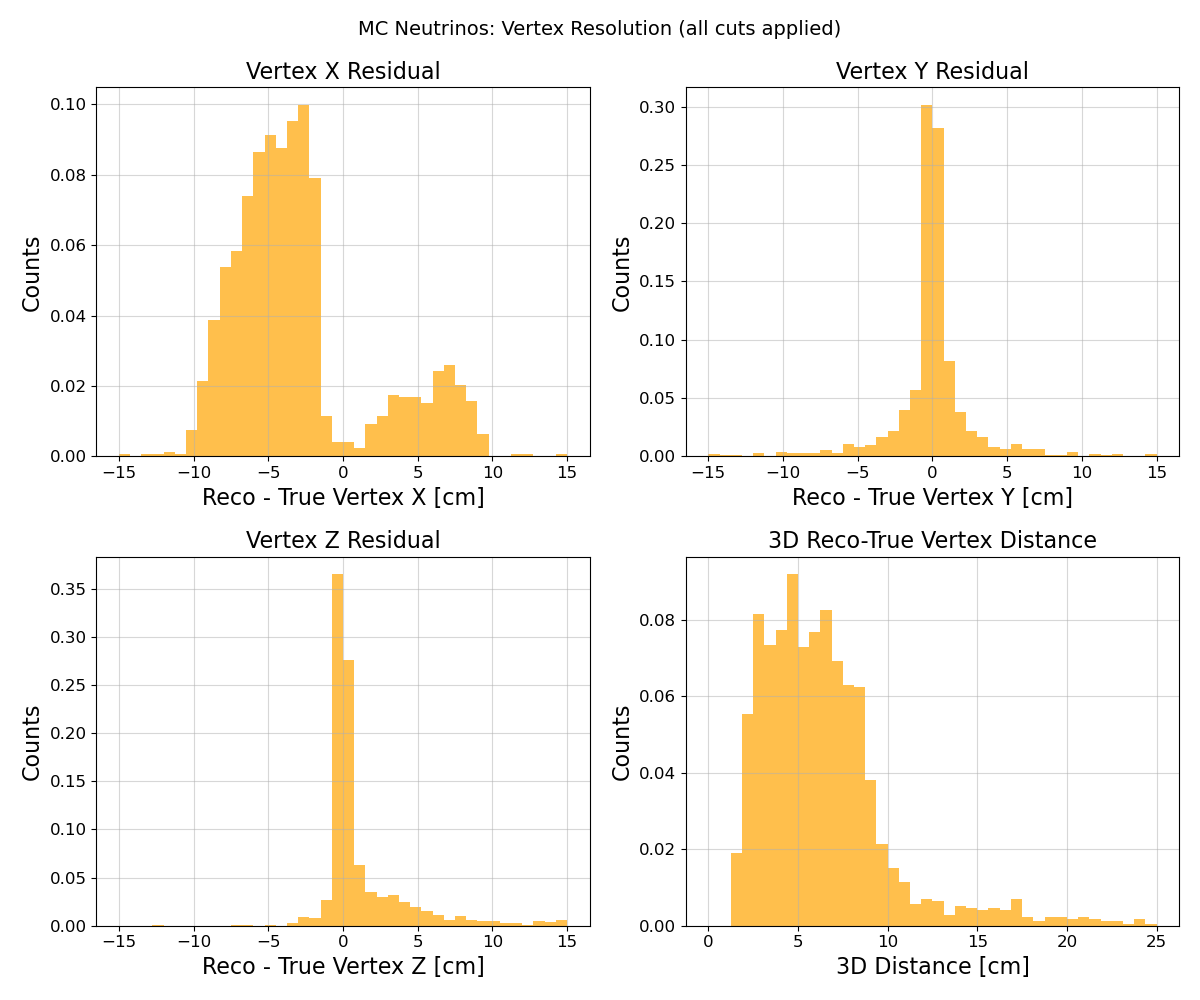
\includegraphics[width=0.87\linewidth]{sections/appendix/changes/mc_vertex_resolution_old.png}
    \caption{Old reconstruction performances, area normalized to 1. Top left: Difference between the reconstructed and true vertex X position. Top right: Difference between the reconstructed and true vertex Y position. Bottom left: Difference between the reconstructed and true vertex Z position. Bottom right: Distance in 3D between the reconstructed and true position.}
    \label{fig:resolution_old}
\end{figure}
\begin{figure}[!h]
    \centering
    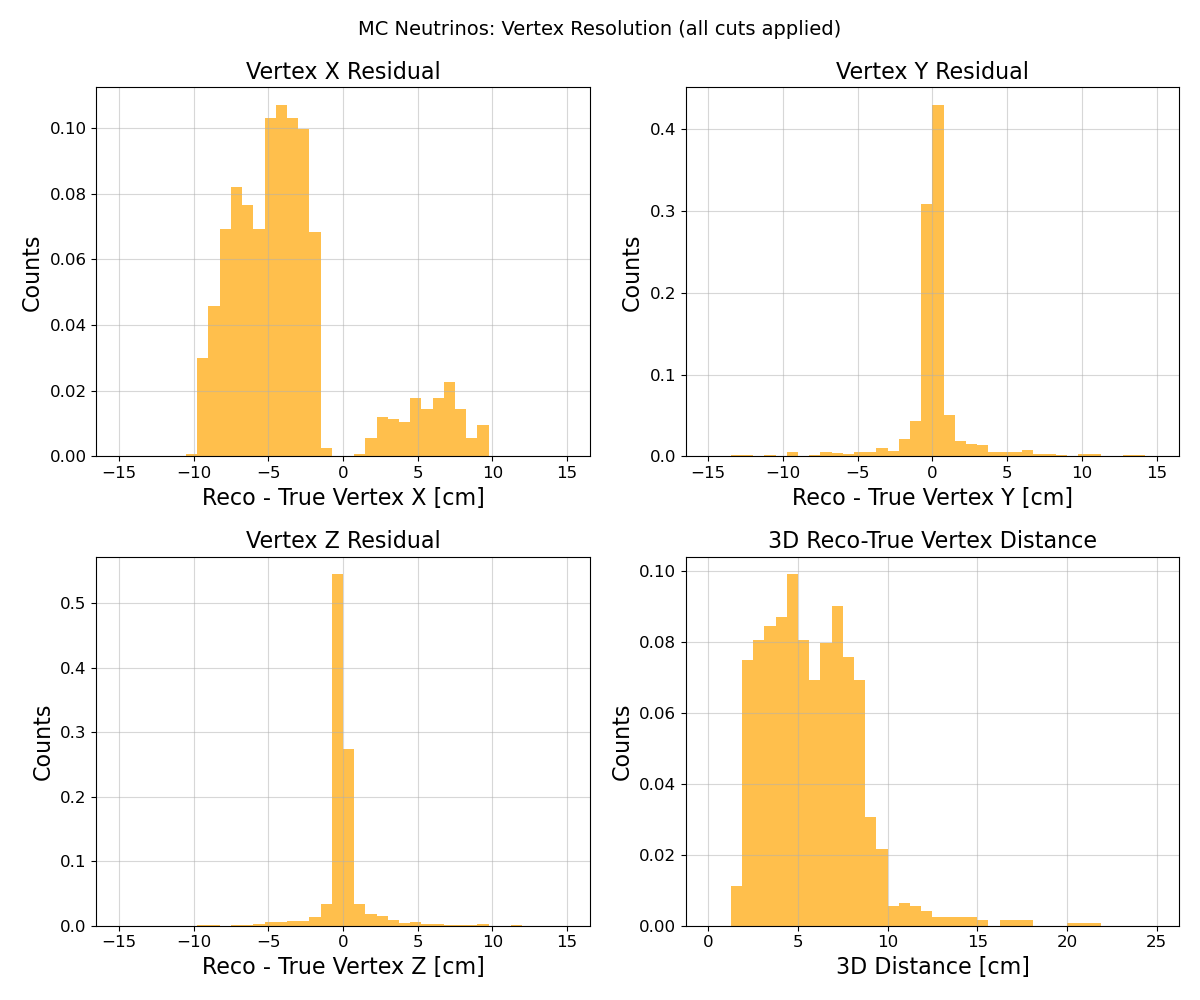
\includegraphics[width=0.87\linewidth]{sections/appendix/changes/mc_vertex_resolution_new.png}
    \caption{New reconstruction performances, area normalized to 1. Top left: Difference between the reconstructed and true vertex X position. Top right: Difference between the reconstructed and true vertex Y position. Bottom left: Difference between the reconstructed and true vertex Z position. Bottom right: Distance in 3D between the reconstructed and true position.}    
    \label{fig:resolution_new}
\end{figure}

The new reconstruction, together with the fixed channel map, improves the vertex position reconstruction significantly, mostly in the Y-Z plane. 


\subsection{Results comparison}
\begin{table}[htbp]
\centering
\resizebox{\textwidth}{!}{%
\begin{tabular}{lccc}
\hline
Cut & Beam-off Events/h & Beam-on Events/h & Beam On/Beam Off Ratio \\
\hline
Before cuts & $1950.26 \pm 6.61$ & $2383.98 \pm 12.01$ & $1.22$ \\
Max $\cos(\theta_{\mathrm{beam}})$ & $106.34 \pm 1.54$ & $217.53 \pm 3.63$ & $2.05$ \\
Tail Length Density & $23.09 \pm 0.72$ & $28.96 \pm 1.32$ & $1.25$ \\
Cut on $C_{140-150}$ & $6.65 \pm 0.39$ & $9.92 \pm 0.77$ & $1.49$ \\
ROI Z close to vertex & $1.79 \pm 0.20$ & $3.87 \pm 0.48$ & $2.16$ \\
N daughter particles & $0.81 \pm 0.13$ & $2.84 \pm 0.41$ & $3.53$ \\
Vertex fiducial volume & $0.65 \pm 0.12$ & $2.48 \pm 0.39$ & $3.82$ \\
Cut on $C_{40-50}$ & $0.56 \pm 0.11$ & $2.36 \pm 0.38$ & $4.21$ \\
ROI Z size & $0.49 \pm 0.10$ & $2.12 \pm 0.36$ & $4.30$ \\
Cut on $C_{0-10}$ & $0.45 \pm 0.10$ & $1.87 \pm 0.34$ & $4.19$ \\
\hline
\end{tabular}
}
\caption{Beam-on and beam-off events per hour with the corresponding ratio for various selection cuts, considering all the available time with the spill on.}
\label{tab:}
\end{table}

\begin{table}[htbp]
\centering
\resizebox{\textwidth}{!}{%
\begin{tabular}{lccc}
\hline
Cut & Beam-off Events/h & Beam-on Events/h & Beam On/Beam Off Ratio \\
\hline
Initial & $2095.37 \pm 6.85$ & $2648.58 \pm 12.65$ & $1.26$ \\
Neutrino PFParticle in slice & $1982.99 \pm 6.66$ & $2498.93 \pm 12.29$ & $1.26$ \\
Vertex fiducial volume & $1163.63 \pm 5.10$ & $1182.32 \pm 8.46$ & $1.02$ \\
N daughter particles & $577.82 \pm 3.60$ & $558.08 \pm 5.81$ & $0.97$ \\
Max $\cos(\theta_{\mathrm{beam}})$ & $54.85 \pm 1.11$ & $68.63 \pm 2.04$ & $1.25$ \\
Cut on $C_{0-10}$ & $21.48 \pm 0.69$ & $25.58 \pm 1.24$ & $1.19$ \\
Cut on $C_{40-50}$ & $15.82 \pm 0.59$ & $18.26 \pm 1.05$ & $1.15$ \\
Cut on $C_{140-150}$ & $8.37 \pm 0.43$ & $12.94 \pm 0.88$ & $1.55$ \\
ROI Z size & $5.37 \pm 0.35$ & $9.73 \pm 0.77$ & $1.81$ \\
ROI Z close to vertex & $2.06 \pm 0.21$ & $5.80 \pm 0.59$ & $2.82$ \\
Tail Length Density & $0.69 \pm 0.12$ & $3.69 \pm 0.47$ & $5.35$ \\
\hline
\end{tabular}
}
\caption{Beam-on and beam-off events per hour with the corresponding ratio for various selection cuts, considering all the available time with the spill on.}
\label{tab:}
\end{table}

